\chapter{Đường trắc địa, gia tốc đều và giới hạn Newton}

Vấn đề trước mắt là hấp dẫn. Nói chính xác hơn, ta muốn metric không-thời gian mô tả một trường hấp dẫn gần như đều, chẳng hạn trường trong một phòng thí nghiệm nhỏ gần bề mặt Trái Đất. Con đường ngắn nhất dẫn tới metric đó hóa ra lại không phải là trực tiếp. Trước hết, ta phải cụ thể hóa về mặt thao tác ba ý tưởng hình học: đạo hàm hiệp biến, phép vận chuyển song song và chuyển động trắc địa.

Những ý tưởng này phụ thuộc lẫn nhau. Đạo hàm hiệp biến cho ta biết cách so sánh các vectơ tại những điểm lân cận. Phép vận chuyển song song cho ta biết cách mang một vectơ đi mà không làm nó quay. Một đường trắc địa thu được khi vectơ đang được mang chính là tiếp tuyến của bản thân đường đi. Khi đường ấy nằm trong không-thời gian thay vì trong không gian, chính phương trình trắc địa đó trở thành phương trình chuyển động của một hạt rơi tự do.

Nửa sau của bài giảng sau đó thực hiện một bước đi nổi bật. Ta vẫn ở trong không-thời gian Minkowski phẳng, nhưng mô tả nó bằng các tọa độ thích nghi với một họ quan sát viên gia tốc cứng. Trong các tọa độ đó, metric mang dáng vẻ hấp dẫn. Gần một quan sát viên, nó tái hiện thế của một trường đều, và các đường trắc địa của nó tuân theo phương trình Newton
\begin{equation}
\frac{d^2y}{d\tau^2}=-g.
\end{equation}
Đây là nguyên lý tương đương được viết ra dưới dạng một phép tính.

\section{Nhắc lại đạo hàm hiệp biến}

Tại một điểm được chọn \(P\), có thể chọn các tọa độ Cartesian nhất có thể. Bài giảng ban đầu dùng cụm từ tọa độ chuẩn Gauss rồi lập tức nói rõ thêm. Tên gọi kém quan trọng hơn các điều kiện cục bộ:
\begin{equation}
g_{mn}(P)=\delta_{mn},
\qquad
\partial_r g_{mn}(P)=0.
\label{eq:l4-normal-point}
\end{equation}
Đây là các tọa độ chuẩn tại một điểm. Chúng không nhất thiết vẫn là Cartesian trong một lân cận hữu hạn, và có nhiều hệ như vậy vì các trục của chúng có thể được quay.

Metric tương thích với toán tử đạo hàm:
\begin{equation}
\nabla_r g_{mn}=0,
\qquad
\nabla_r g^{mn}=0.
\label{eq:l4-metric-compatibility}
\end{equation}
Đối với một đối vectơ \(V_s\), đạo hàm hiệp biến là
\begin{equation}
\nabla_r V_s
=
\partial_r V_s-\Gamma^p{}_{rs}V_p.
\label{eq:l4-covector-derivative}
\end{equation}
Các hệ số liên thông là
\begin{equation}
\Gamma^p{}_{rs}
=
\frac{1}{2}g^{pn}
\left(
\partial_s g_{nr}
+\partial_r g_{ns}
-\partial_n g_{rs}
\right).
\label{eq:l4-christoffel}
\end{equation}
Một vài chỉ số được chỉnh lại trong lúc biểu thức này được viết trên bảng. Phương trình \eqref{eq:l4-christoffel} là hệ thức đã hoàn chỉnh. Nó đối xứng theo \(r\) và \(s\), đúng như mong đợi đối với liên thông Levi-Civita không xoắn.

\begin{figure}[htbp]
\centering
\includegraphics[width=0.92\textwidth]{lecture_04_figure_01.png}
\caption{Đạo hàm của đối vectơ và công thức đầy đủ của ký hiệu Christoffel.}
\end{figure}

Vì các ký hiệu Christoffel được tạo từ các đạo hàm bậc nhất của metric, nên chúng triệt tiêu tại \(P\) trong các tọa độ \eqref{eq:l4-normal-point}. Chúng không triệt tiêu trong mọi hệ tọa độ, ngay cả khi không gian nền là phẳng. Do đó \(\Gamma^p{}_{rs}\) không phải là một tensor. Chính tính không tensor ấy về sau sẽ cho phép một quan sát viên gia tốc mô tả một lực hấp dẫn mà một quan sát viên quán tính không thấy.

\subsection{Nâng chỉ số của vectơ}

Đạo hàm tương ứng của một vectơ không được đưa vào như một quy tắc riêng cần ghi nhớ. Nó suy ra từ metric. Bắt đầu với
\begin{equation}
V^n=g^{np}V_p.
\end{equation}
Khi đó
\begin{align}
\nabla_m V^n
&=\nabla_m\!\left(g^{np}V_p\right) \\
&=(\nabla_m g^{np})V_p+g^{np}\nabla_m V_p \\
&=g^{np}\left(\partial_mV_p-\Gamma^r{}_{mp}V_r\right),
\end{align}
ở đó tính tương thích metric đã loại bỏ hạng thứ nhất. Sắp xếp lại các chỉ số cho ta
\begin{equation}
\nabla_m V^n
=
\partial_m V^n+\Gamma^n{}_{mr}V^r.
\label{eq:l4-vector-derivative}
\end{equation}

\begin{figure}[htbp]
\centering
\includegraphics[width=0.90\textwidth]{lecture_04_figure_02.png}
\caption{Nâng chỉ số bằng metric nghịch đảo trước khi lấy đạo hàm.}
\end{figure}

\begin{figure}[htbp]
\centering
\includegraphics[width=0.90\textwidth]{lecture_04_figure_03.png}
\caption{Đạo hàm với chỉ số trên xuất hiện từ tính tương thích metric và quy tắc tích.}
\end{figure}

Ngữ pháp của các chỉ số vì thế rất đơn giản:
\begin{equation}
\boxed{
\begin{aligned}
\text{lower index:}&\quad -\Gamma,\\
\text{upper index:}&\quad +\Gamma.
\end{aligned}}
\end{equation}
Đối với một tensor hạng cao hơn, có một hạng liên thông xuất hiện cho mỗi chỉ số, với dấu của nó được quyết định bởi việc chỉ số đó ở dưới hay ở trên.

\subsection{Một câu hỏi về thuật ngữ}

Chính xác thì các tọa độ tốt nhất được nhắc ở trên là gì? Ở đây không hề khẳng định đó là một hệ tọa độ toàn cục đặc biệt. Tại một điểm được chọn, chúng làm cho metric bằng dạng phẳng của nó và làm cho các đạo hàm bậc nhất của metric triệt tiêu. Quay các trục đi sẽ cho một hệ quy chiếu khác cũng tốt như vậy. Các mệnh đề hình học suy ra trong một hệ như thế không phụ thuộc vào định hướng ấy, vì các đối tượng cuối cùng thu được là tensor.

\section{Vận chuyển song song dọc theo một đường cong}

Giả sử một vectơ \(V^n\) được mang dọc theo một đường cong. Qua một độ dời vô cùng bé \(dx^m\), độ biến thiên hiệp biến của nó là
\begin{align}
\delta V^n
&=(\nabla_mV^n)\,dx^m \\
&=\partial_mV^n\,dx^m
+\Gamma^n{}_{mr}V^r\,dx^m \\
&=dV^n+\Gamma^n{}_{mr}V^r\,dx^m.
\label{eq:l4-covariant-differential}
\end{align}

\begin{figure}[htbp]
\centering
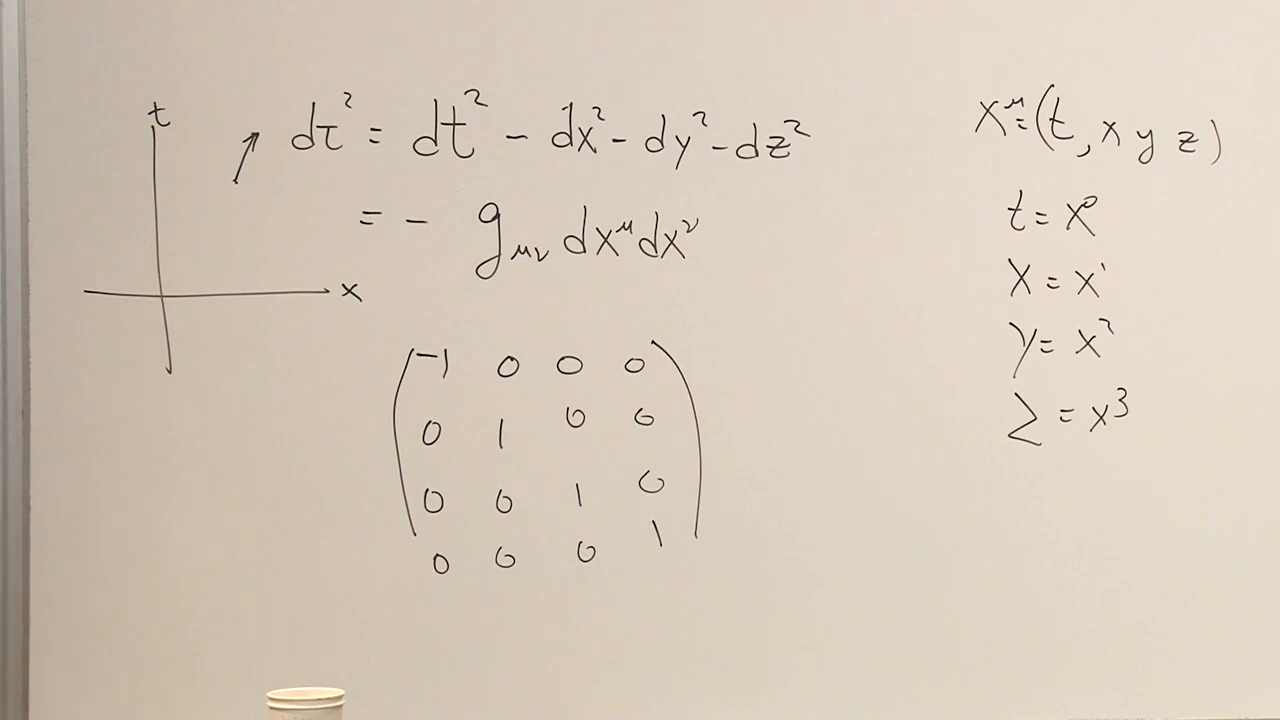
\includegraphics[width=0.92\textwidth]{lecture_04_figure_04.png}
\caption{Sự thay đổi thành phần thông thường và hiệu chỉnh liên thông dọc theo một đường cong.}
\end{figure}

Vectơ được vận chuyển song song khi độ biến thiên hiệp biến này triệt tiêu:
\begin{equation}
\boxed{
dV^n+\Gamma^n{}_{mr}V^r\,dx^m=0.
}
\label{eq:l4-parallel-transport}
\end{equation}
Về mặt thao tác, ta có thể hình dung dựng một hệ quy chiếu chuẩn tại mỗi điểm của đường cong. Trong hệ cục bộ đó, vectơ được vận chuyển được yêu cầu là không quay. Sau đó ta đi một khoảng vô cùng bé, dựng hệ quy chiếu chuẩn kế tiếp, rồi lặp lại.

\begin{figure}[htbp]
\centering
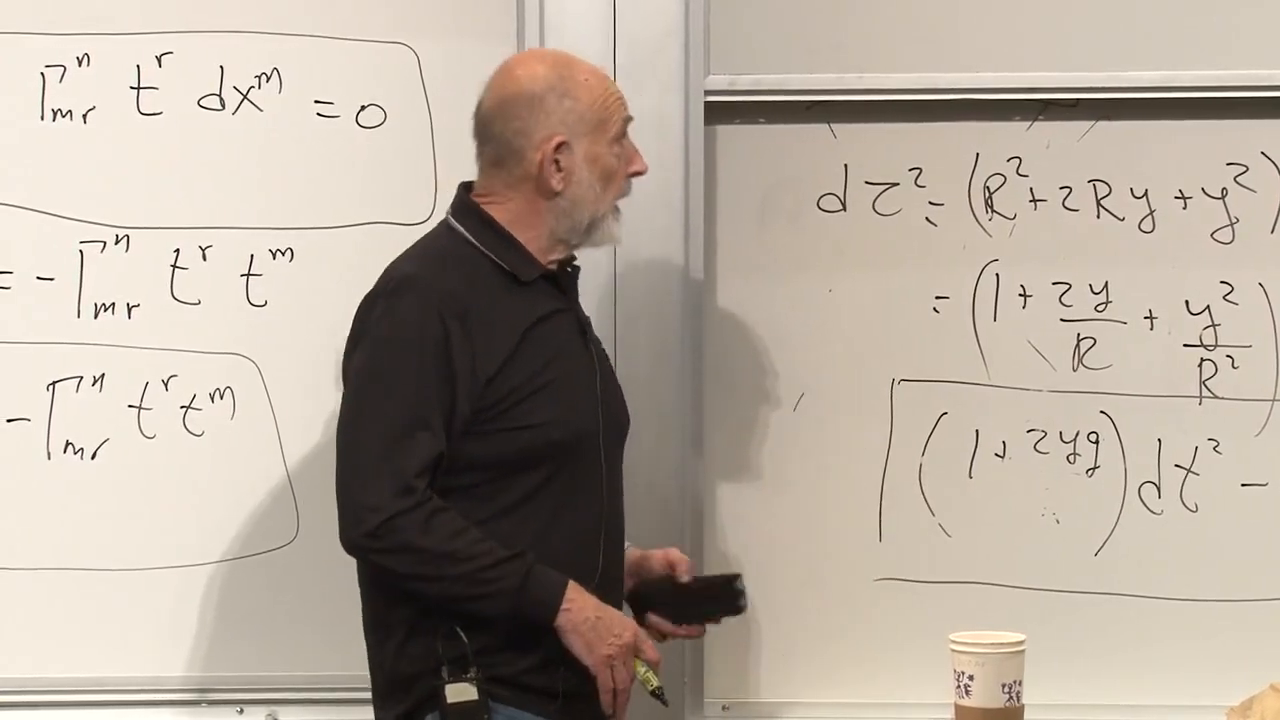
\includegraphics[width=0.92\textwidth]{lecture_04_figure_05.png}
\caption{Dạng phương trình vận chuyển song song được viết rõ trên bảng.}
\end{figure}

Định hướng của mỗi hệ quy chiếu chuẩn tạm thời không thuộc nội dung vật lý. Ta có thể quay nó trước khi thực hiện phép so sánh. Điều quan trọng là mệnh đề hiệp biến \eqref{eq:l4-parallel-transport} độc lập với lựa chọn tùy ý đó.

\subsection{Sự phụ thuộc vào đường đi và độ cong}

Trong một không gian cong, phép vận chuyển song song phụ thuộc vào đường đi. Hãy bắt đầu với cùng một vectơ tại cùng một điểm đầu và vận chuyển nó tới cùng một điểm cuối theo hai lộ trình khác nhau. Nói chung, các vectơ cuối cùng sẽ khác nhau. Vận chuyển một vectơ quanh một vòng kín có thể trả nó về trong trạng thái đã bị quay. Sự sai khác đó là holonomy, và nó là một dấu hiệu trực tiếp của độ cong.

\begin{figure}[htbp]
\centering
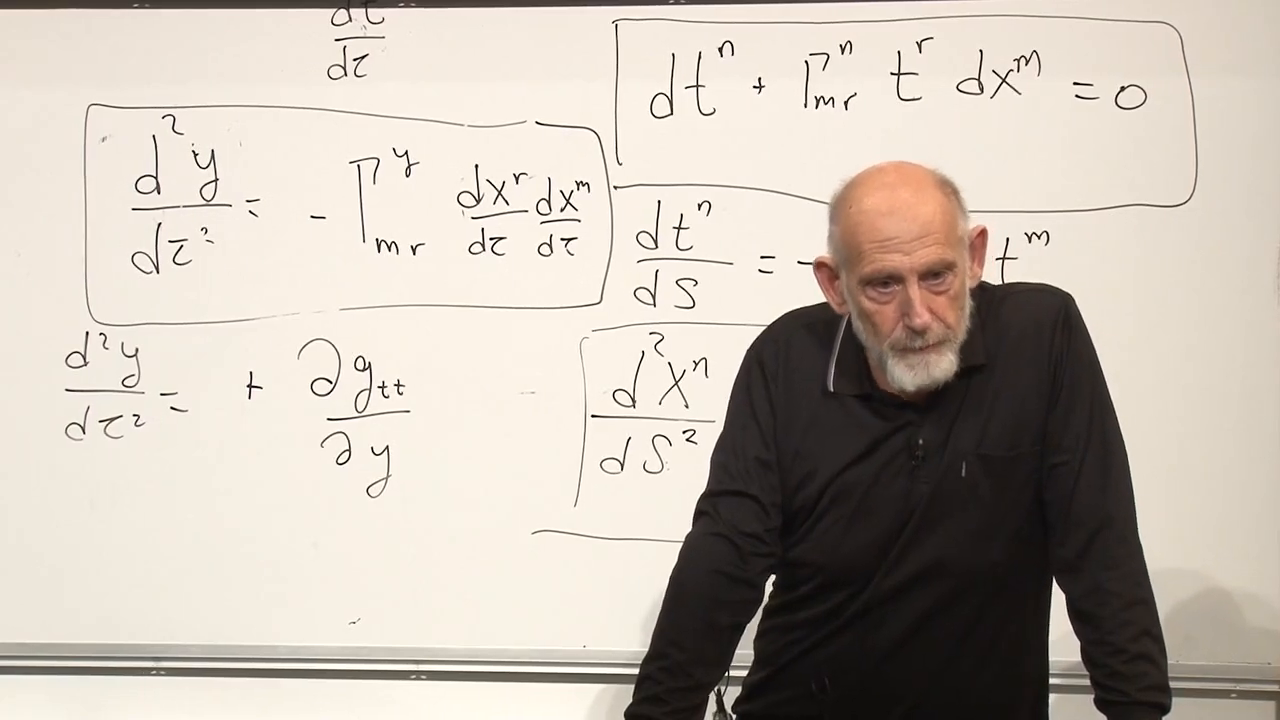
\includegraphics[width=0.90\textwidth]{lecture_04_figure_06.png}
\caption{Hai lộ trình trên một mặt cong không nhất thiết vận chuyển một vectơ tới cùng một định hướng cuối cùng.}
\end{figure}

Hình nón cho một ví dụ hữu ích. Xa đỉnh của nó, một hình nón có thể được cắt mở và trải phẳng. Tuy vậy, vận chuyển song song quanh một vòng kín bao lấy đỉnh vẫn trả vectơ về sau khi quay đi một góc bằng độ thiếu hụt góc. Nếu đỉnh được bo tròn, độ cong là hữu hạn và trải ra trên một vùng nhỏ. Nếu nó nhọn hoàn toàn, sự lý tưởng hóa sẽ tập trung độ cong tại đỉnh.

\begin{figure}[htbp]
\centering
\includegraphics[width=0.90\textwidth]{lecture_04_figure_07.png}
\caption{Chuyển động tròn trên hình nón và biểu diễn phẳng của nó sau khi cắt mở.}
\end{figure}

\subsection{Các câu hỏi về vectơ được vận chuyển}

\paragraph{Vectơ có phải được xác định ở mọi nơi không?}
Không. Ta có thể bắt đầu với một vectơ đơn lẻ tại một điểm và chỉ giải \eqref{eq:l4-parallel-transport} dọc theo đường cong đã chọn. Một trường vectơ đầy đủ là không bắt buộc. Nếu một trường đã được xác định trên một vùng, nó có thể hằng hiệp biến theo một hướng mà không theo hướng khác.

\paragraph{Độ dài của nó có được bảo toàn không?}
Có. Đặt \(V^2=g_{mn}V^mV^n\). Dọc theo đường cong,
\begin{align}
\frac{D}{d\lambda}\left(g_{mn}V^mV^n\right)
&=
\frac{Dg_{mn}}{d\lambda}V^mV^n
+2g_{mn}V^m\frac{DV^n}{d\lambda}\\
&=0.
\end{align}
Tính tương thích metric làm hạng thứ nhất triệt tiêu, còn vận chuyển song song làm hạng thứ hai triệt tiêu. Vì thế, các độ dài và các góc giữa những vectơ được vận chuyển song song đều được bảo toàn.

\paragraph{Vectơ tiếp tuyến của mọi đường cong có được vận chuyển song song không?}
Không. Câu hỏi này dẫn thẳng tới các đường trắc địa. Vectơ tiếp tuyến của một lộ trình tròn quanh hình nón quay liên tục. Còn tiếp tuyến của đường thẳng thu được sau khi cắt mở hình nón thì không. Chỉ đường thứ hai mới thẳng cục bộ.

\section{Đường trắc địa: thẳng nhất chứ không chỉ ngắn nhất}

Một đường trắc địa có hai mô tả liên hệ với nhau. Xét toàn cục, nó là một đường làm dừng phiếm hàm độ dài hoặc thời gian riêng. Xét cục bộ, nó là đường thẳng nhất có thể. Từ dừng là quan trọng: tùy vào hình học và các điểm mút, đường đó không nhất thiết là cực tiểu toàn cục duy nhất. Trong không-thời gian Lorentz, các đường trắc địa kiểu thời cục bộ cực đại hóa thời gian riêng chứ không cực tiểu hóa một khoảng cách dương.

Mô tả cục bộ là mô tả cần dùng ở đây. Một chiếc xe nhỏ chạy trên địa hình cong với vô lăng giữ thẳng hẳn về phía trước sẽ đi theo một đường trắc địa, miễn là xe đủ nhỏ so với thang độ uốn cong của địa hình. Nó không nhất thiết trông thẳng trong một không gian nhúng; nó thẳng theo hình học sẵn có trên bề mặt.

\begin{figure}[htbp]
\centering
\includegraphics[width=0.90\textwidth]{lecture_04_figure_08.png}
\caption{Một đường được vẽ theo cách nội tại trên mặt cong, chuẩn bị cho định nghĩa về đường thẳng nhất.}
\end{figure}

\subsection{Vectơ tiếp tuyến}

Cho đường cong là \(x^m(s)\), với độ dài cung
\begin{equation}
ds^2=g_{mn}\,dx^m dx^n.
\end{equation}
Véc-tơ tiếp tuyến đơn vị là
\begin{equation}
t^m=\frac{dx^m}{ds}.
\label{eq:l4-unit-tangent}
\end{equation}
Về mặt hình học, lấy hai điểm gần nhau, lập véc-tơ độ dời nối chúng, chia cho khoảng cách giữa chúng, rồi cho hai điểm tiến đến trùng nhau.

\begin{figure}[htbp]
\centering
\includegraphics[width=0.90\textwidth]{lecture_04_figure_09.png}
\caption{Hướng tiếp tuyến là giới hạn của độ dời dọc theo một đường cong.}
\end{figure}

\begin{figure}[htbp]
\centering
\includegraphics[width=0.90\textwidth]{lecture_04_figure_10.png}
\caption{Phần tử độ dài và véc-tơ tiếp tuyến đơn vị \(t^m=dx^m/ds\).}
\end{figure}

Đường trắc địa là một đường cong mà véc-tơ tiếp tuyến của nó được chuyển song song dọc theo chính nó:
\begin{equation}
dt^n+\Gamma^n{}_{mr}t^r\,dx^m=0.
\end{equation}
Chia cho \(ds\) và dùng \(dx^m/ds=t^m\):
\begin{equation}
\frac{dt^n}{ds}
=
-\Gamma^n{}_{mr}t^m t^r.
\end{equation}
Cuối cùng thay \(t^n=dx^n/ds\) vào:
\begin{equation}
\boxed{
\frac{d^2x^n}{ds^2}
+\Gamma^n{}_{mr}
\frac{dx^m}{ds}
\frac{dx^r}{ds}
=0.
}
\label{eq:l4-geodesic}
\end{equation}

\begin{figure}[htbp]
\centering
\includegraphics[width=0.94\textwidth]{lecture_04_figure_11.png}
\caption{Quy luật chuyển song song của véc-tơ tiếp tuyến và phương trình trắc địa bậc hai.}
\end{figure}

Phương trình \eqref{eq:l4-geodesic} đã khá giống động lực học Newton. Nếu \(s\) được thay bằng một tham số thời gian thích hợp, hạng thứ nhất là một gia tốc. Hạng liên kết khi đó tác dụng như một lực trên đơn vị khối lượng, được quyết định hoàn toàn bởi metric. Trong thuyết tương đối rộng, phép tương tự này trở thành đúng theo nghĩa đen: các hạt tự do đi theo các đường trắc địa của không-thời gian, và đại lượng mà Newton gọi là gia tốc hấp dẫn xuất hiện thông qua liên kết.

\section{Từ khoảng cách Riemann đến thời gian riêng trong không-thời gian}

Giờ đây phần thảo luận chuyển từ không gian cong sang không-thời gian. Trong các tọa độ Descartes quán tính, thời gian riêng giữa các sự kiện lân cận là
\begin{equation}
d\tau^2
=dt^2-dx^2-dy^2-dz^2.
\label{eq:l4-proper-time}
\end{equation}
Bài giảng dùng
\begin{equation}
d\tau^2=-g_{\mu\nu}\,dx^\mu dx^\nu
\label{eq:l4-lecture-sign}
\end{equation}
với
\begin{equation}
g_{\mu\nu}
=
\eta_{\mu\nu}
=
\begin{pmatrix}
-1&0&0&0\\
0&1&0&0\\
0&0&1&0\\
0&0&0&1
\end{pmatrix}.
\label{eq:l4-eta}
\end{equation}
Vì vậy, dấu trừ ở ngoài trong \eqref{eq:l4-lecture-sign} biến metric với quy ước chủ yếu dấu cộng đã chọn thành \eqref{eq:l4-proper-time}. Các tọa độ là
\begin{equation}
\begin{aligned}
x^\mu&=(t,x,y,z),\\
x^0&=t,\quad x^1=x,\\
x^2&=y,\quad x^3=z.
\end{aligned}
\end{equation}

\begin{figure}[htbp]
\centering
\includegraphics[width=0.94\textwidth]{lecture_04_figure_12.png}
\caption{Thời gian riêng, các tọa độ không-thời gian và metric Minkowski với quy ước chủ yếu dấu cộng.}
\end{figure}

Chữ ký là thông tin bất biến: một trị riêng mang dấu gắn với thời gian và ba trị riêng mang dấu gắn với không gian. Nhân toàn bộ metric với \(-1\) và điều chỉnh nhất quán mọi quy ước sẽ cho quy ước chủ yếu dấu trừ cũng phổ biến không kém. Không có nội dung vật lý nào phụ thuộc vào lựa chọn tổng thể đó.

Bài giảng đặt câu hỏi liệu các không gian có những chữ ký không xác định khác đã từng được xem xét hay chưa. Về mặt toán học, các hình học giả Riemann với nhiều chữ ký khác nhau đã được thiết lập vững chắc. Điểm vật lý thì hẹp hơn: không-thời gian tương đối tính quan sát được là Lorentz, với một hướng thời gian. Các hướng kiểu thời gian bổ sung sẽ làm thay đổi sâu sắc cấu trúc nhân quả và không mô tả nền vật lý đang được bàn tới.

\begin{figure}[htbp]
\centering
\includegraphics[width=0.94\textwidth]{lecture_04_figure_13.png}
\caption{Quy ước dấu được kiểm tra trước khi \(\eta_{\mu\nu}\) được dùng để ký hiệu metric phẳng.}
\end{figure}

Không-thời gian phẳng không có nghĩa là các thành phần của metric phải có dạng \(\eta_{\mu\nu}\) trong mọi hệ tọa độ. Nó có nghĩa là tồn tại những tọa độ mà trong đó chúng có dạng ấy. Các tọa độ cong tuyến hoặc gia tốc có thể làm các thành phần biến thiên theo vị trí ngay cả khi tensor Riemann bằng 0.

\section{Vì sao gia tốc tọa độ như nhau không giữ được độ cứng}

Ta muốn có các tọa độ gắn với một thang máy đang gia tốc. Ý tưởng đầu tiên là xếp một dãy người quan sát ở những khoảng cách cố định với nhau và cho tất cả họ cùng một gia tốc tọa độ. Thuyết tương đối ngăn không cho cách dựng ngây thơ ấy duy trì được tính cứng.

\begin{figure}[htbp]
\centering
\includegraphics[width=0.92\textwidth]{lecture_04_figure_14.png}
\caption{Một hàng những người quan sát lân cận dùng để kiểm tra xem một gia tốc chung có bảo toàn độ cứng hay không.}
\end{figure}

Nếu các người quan sát tách biệt tuân theo những chương trình gia tốc giống hệt nhau theo một hệ quy chiếu quán tính, thì khoảng cách giữa họ, đo trong các hệ nghỉ tức thời đang thay đổi của họ, không giữ cố định. Một sợi dây nối họ sẽ bị kéo giãn và cuối cùng đứt. Đây chính là cùng sức căng động học xuất hiện trong thí nghiệm tưởng tượng tàu vũ trụ Bell. Hơn nữa, gia tốc tọa độ Newton không đổi không thể tiếp diễn vô hạn: rốt cuộc nó sẽ dự đoán một tốc độ lớn hơn tốc độ ánh sáng.

Vì vậy, một hệ quy chiếu gia tốc cứng theo thuyết tương đối phải dùng một gia tốc riêng khác nhau tại mỗi vị trí. Những người quan sát ở gần chân trời sắp xuất hiện hơn thì gia tốc mạnh hơn; những người ở xa hơn thì gia tốc nhẹ hơn. Khi đó, các khoảng cách riêng giữa họ có thể giữ không đổi trong hệ quy chiếu đồng chuyển động tức thời. Đây là gia tốc cứng Born trong một chiều không gian.

\section{Tọa độ cực Euclid làm bước khởi động}

Cách dựng đúng dễ thấy nhất khi bắt đầu từ một đường tròn thông thường. Trên mặt phẳng Euclid,
\begin{equation}
x=r\cos\theta,
\qquad
y=r\sin\theta,
\end{equation}
nên
\begin{equation}
x^2+y^2=r^2,
\qquad
\cos^2\theta+\sin^2\theta=1.
\end{equation}
Các dạng mũ phức là
\begin{equation}
\cos\theta=\frac{e^{i\theta}+e^{-i\theta}}{2},
\qquad
\sin\theta=\frac{e^{i\theta}-e^{-i\theta}}{2i}.
\label{eq:l4-euler-trig}
\end{equation}
Thừa số \(i\) ở mẫu số của công thức sin được phát hiện là bị thiếu và được khôi phục lại trong lúc thảo luận trên bảng.

\begin{figure}[htbp]
\centering
\includegraphics[width=0.94\textwidth]{lecture_04_figure_15.png}
\caption{Đường tròn, các tọa độ cực Euclid và các dạng lượng giác mũ của chúng.}
\end{figure}

Một giá trị cố định của \(r\) là một đường tròn. Chuyển động với tốc độ góc không đổi có gia tốc hướng tâm có độ lớn không đổi, luôn hướng vào trong. Trong không-thời gian, hyperbol sẽ đóng vai trò tương ứng.

\section{Tọa độ hyperbol trong không-thời gian Minkowski}

Thay các hàm lượng giác bằng các hàm hyperbol tương ứng:
\begin{equation}
\cosh\omega=\frac{e^\omega+e^{-\omega}}{2},
\qquad
\sinh\omega=\frac{e^\omega-e^{-\omega}}{2},
\end{equation}
với
\begin{equation}
\cosh^2\omega-\sinh^2\omega=1.
\label{eq:l4-hyperbolic-identity}
\end{equation}
Không có thừa số \(i\). Tọa độ \(\omega\) là một góc hyperbol, hay độ nhanh. Không giống một góc thông thường, nó không tuần hoàn; nó chạy từ \(-\infty\) đến \(+\infty\).

\begin{figure}[htbp]
\centering
\includegraphics[width=0.94\textwidth]{lecture_04_figure_16.png}
\caption{Trong phép dựng không-thời gian, các hàm lượng giác được thay bằng các hàm hyperbol.}
\end{figure}

Định nghĩa các tọa độ mới trong miền nêm Rindler phải:
\begin{equation}
x=r\cosh\omega,
\qquad
t=r\sinh\omega,
\qquad
r>0.
\label{eq:l4-rindler-transform}
\end{equation}
Khi đó
\begin{equation}
x^2-t^2=r^2.
\label{eq:l4-rindler-hyperbola}
\end{equation}
Với \(r\) cố định, cho \(\omega\) biến thiên sẽ vạch ra một hyperbol. Khi \(r\) tăng, ta đi qua họ ấy theo một hướng kiểu không gian, còn khi \(\omega\) tăng, ta tiến về phía trước dọc theo một hyperbol theo một hướng kiểu thời gian.

\begin{figure}[htbp]
\centering
\includegraphics[width=0.94\textwidth]{lecture_04_figure_17.png}
\caption{Phép biến đổi tọa độ \(x=r\cosh\omega\), \(t=r\sinh\omega\) và hyperbol bất biến của nó.}
\end{figure}

\begin{figure}[htbp]
\centering
\includegraphics[width=0.94\textwidth]{lecture_04_figure_18.png}
\caption{Một họ các hyperbol \(r\) cố định biểu diễn một tập hợp gia tốc cứng.}
\end{figure}

\subsection{Metric trong các tọa độ gia tốc}

Lấy vi phân của \eqref{eq:l4-rindler-transform}:
\begin{align}
dx&=\cosh\omega\,dr+r\sinh\omega\,d\omega,\\
dt&=\sinh\omega\,dr+r\cosh\omega\,d\omega.
\end{align}
Dùng \eqref{eq:l4-hyperbolic-identity}, các hạng chéo triệt tiêu:
\begin{align}
d\tau^2
&=dt^2-dx^2\\
&=r^2\,d\omega^2-dr^2.
\label{eq:l4-rindler-metric}
\end{align}
Các hướng ngang, khi được khôi phục, chỉ đơn giản cộng thêm \(-dy^2-dz^2\) vào quy ước thời gian riêng được dùng ở đây.

Đây vẫn là không-thời gian phẳng. Hệ số phụ thuộc tọa độ \(r^2\) không phải là bằng chứng của độ cong hơn gì so với \(r^2\) nhân với \(d\theta^2\) trong tọa độ cực Euclid.

\subsection{Gia tốc riêng dọc theo các hyperbol}

Đối với một đường thế giới cố định \(r=R\), phương trình \eqref{eq:l4-rindler-metric} cho
\begin{equation}
d\tau=R\,d\omega.
\end{equation}
Vận tốc bốn chiều của nó là
\begin{equation}
U^\mu
=
\frac{d(t,x)}{d\tau}
=
(\cosh\omega,\sinh\omega),
\end{equation}
và gia tốc bốn chiều của nó là
\begin{equation}
A^\mu
=
\frac{dU^\mu}{d\tau}
=
\frac{1}{R}(\sinh\omega,\cosh\omega).
\end{equation}
Độ lớn bất biến là hằng số:
\begin{equation}
a=\sqrt{A^\mu A_\mu}=\frac{1}{R}
\qquad (c=1).
\label{eq:l4-proper-acceleration}
\end{equation}

\begin{figure}[htbp]
\centering
\includegraphics[width=0.90\textwidth]{lecture_04_figure_19.png}
\caption{Quy luật nghịch đảo theo bán kính \(a=1/R\) cho một đường thế giới gia tốc cố định.}
\end{figure}

Khi khôi phục đơn vị,
\begin{equation}
\boxed{a=\frac{c^2}{R}.}
\label{eq:l4-proper-acceleration-units}
\end{equation}

\begin{figure}[htbp]
\centering
\includegraphics[width=0.90\textwidth]{lecture_04_figure_20.png}
\caption{Khôi phục đơn vị biến \(1/R\) thành \(c^2/R\).}
\end{figure}

Đoạn chắn \(R\) càng nhỏ thì đường thế càng cong gắt và gia tốc riêng mà người quan sát trên đó cảm nhận càng lớn. Các hyperbol ở xa hơn cong ít hơn và đòi hỏi gia tốc nhỏ hơn. Mỗi người quan sát có gia tốc không đổi theo thời gian, nhưng những người quan sát khác nhau lại có các gia tốc khác nhau. Chính sự biến thiên đó bảo toàn các khoảng cách riêng lẫn nhau của họ.

\subsection{Các câu hỏi về hệ tọa độ gia tốc}

\paragraph{Có phải \(R\) là đoạn chắn trên trục \(x\) không?}
Đúng. Tại \(\omega=0\), phương trình \eqref{eq:l4-rindler-transform} cho \(t=0\) và \(x=R\). Đoạn chắn này xác định gia tốc riêng thông qua \eqref{eq:l4-proper-acceleration-units}.

\paragraph{Cách dựng này có phụ thuộc vào gốc tọa độ được chọn không?}
Các tọa độ thì có. Tịnh tiến gốc tọa độ tạo ra một họ hyperbol khác với các tiệm cận bị dời đi. Không có vật lý bất biến nào phụ thuộc vào lựa chọn đó. Ở đây chúng ta chủ ý chọn một hệ tọa độ gia tốc và hỏi chuyển động quán tính xuất hiện như thế nào khi được mô tả trong hệ ấy.

\paragraph{Gia tốc riêng là gì?}
Đó là gia tốc được đo bởi một gia tốc kế mang theo cùng người quan sát. Dưới dạng hiệp biến,
\begin{equation}
A^\mu=\frac{dU^\mu}{d\tau},
\qquad
U^\mu=\frac{dx^\mu}{d\tau}.
\end{equation}
Độ lớn của nó là lực đẩy mà người quan sát thực sự cảm nhận, chứ không phải gia tốc tọa độ \(d^2x/dt^2\) do một hệ quy chiếu ở xa gán cho.

\section{Các metric phẳng trong tọa độ cực và tọa độ hyperbol}

Trước khi xét cục bộ gần Trái Đất, sẽ hữu ích nếu đặt metric Euclid và metric Lorentz cạnh nhau. Trên mặt phẳng,
\begin{equation}
ds^2=dr^2+r^2d\theta^2,
\qquad
g_{ab}
=
\begin{pmatrix}
1&0\\
0&r^2
\end{pmatrix}.
\label{eq:l4-polar-metric}
\end{equation}
Một gợi ý từ người nghe thoáng đưa vào một thừa số dạng cầu, nhưng ở đây chỉ là một mặt phẳng, không phải một mặt cầu. Hạng \(r^2\) ghi nhận thực tế rằng một khoảng góc cố định chắn một cung dài hơn khi bán kính lớn hơn.

\begin{figure}[htbp]
\centering
\includegraphics[width=0.94\textwidth]{lecture_04_figure_21.png}
\caption{Metric cực Euclid: các thành phần phụ thuộc vị trí trên một mặt phẳng vẫn phẳng.}
\end{figure}

Phần tương tự trong Minkowski là
\begin{equation}
d\tau^2=r^2d\omega^2-dr^2.
\end{equation}
Cả hai metric đều có các thành phần phụ thuộc vị trí, nhưng cả hai hình học đều phẳng. Độ cong tọa độ và độ cong hình học không phải là cùng một thứ.

\section{Xét cục bộ gần gia tốc trên Trái Đất}

Chọn một hyperbol mốc sao cho gia tốc riêng của nó bằng giá trị trên Trái Đất \(g\):
\begin{equation}
g=\frac{c^2}{R},
\qquad
R=\frac{c^2}{g}.
\label{eq:l4-earth-radius}
\end{equation}

\begin{figure}[htbp]
\centering
\includegraphics[width=0.94\textwidth]{lecture_04_figure_22.png}
\caption{Chọn hyperbol mốc bằng điều kiện \(c^2/R=g\).}
\end{figure}

Về mặt số,
\begin{equation}
R
\simeq
\frac{(3.0\times10^8\ {\rm m\,s^{-1}})^2}
{9.8\ {\rm m\,s^{-2}}}
\simeq
9.2\times10^{15}\ {\rm m}.
\end{equation}
Bài giảng làm tròn giá trị này thành \(10^{16}\) mét. Một trường bằng một \(g\) trên Trái Đất là nhỏ theo các thang đo tương đối tính, nên bán kính Rindler tương ứng là khổng lồ.

Bây giờ chỉ xét một lân cận nhỏ của người quan sát mốc đó. Đưa vào độ cao cục bộ \(y\) theo
\begin{equation}
r=R+y,
\qquad
dr=dy,
\qquad
|y|\ll R.
\label{eq:l4-local-height}
\end{equation}
Đẳng thức \(dr=dy\) được nêu rõ trong lúc thảo luận, nên hạng không gian phải được viết là \(-dy^2\).

Thế vào \eqref{eq:l4-rindler-metric} thu được
\begin{align}
d\tau^2
&=(R+y)^2d\omega^2-dy^2\\
&=(R^2+2Ry+y^2)d\omega^2-dy^2\\
&=
\left(
1+\frac{2y}{R}+\frac{y^2}{R^2}
\right)
R^2d\omega^2-dy^2.
\label{eq:l4-local-expand}
\end{align}

\begin{figure}[htbp]
\centering
\includegraphics[width=0.94\textwidth]{lecture_04_figure_23.png}
\caption{Khai triển metric gia tốc quanh \(r=R+y\).}
\end{figure}

Định nghĩa một tọa độ thời gian cục bộ
\begin{equation}
t=R\omega.
\label{eq:l4-local-time}
\end{equation}
Khi đó
\begin{equation}
d\tau^2
=
\left(
1+\frac{2y}{R}+\frac{y^2}{R^2}
\right)dt^2-dy^2.
\label{eq:l4-local-exact}
\end{equation}

\begin{figure}[htbp]
\centering
\includegraphics[width=0.94\textwidth]{lecture_04_figure_24.png}
\caption{Đưa vào \(t=R\omega\) sau khi khai triển quanh hyperbol mốc.}
\end{figure}

Ngay cả một độ dịch chuyển theo phương thẳng đứng cỡ vài chục kilômét cũng rất nhỏ so với \(R\). Bài giảng dùng một quãng rơi khoảng 24 dặm để làm cho sự so sánh trở nên trực quan: một khoảng cách như vậy vẫn không đáng kể so với \(10^{16}\) mét. Vì thế \(y^2/R^2\) nhỏ hơn nhiều so với \(y/R\), và có thể bỏ hạng bậc hai:
\begin{equation}
d\tau^2
\simeq
\left(1+\frac{2y}{R}\right)dt^2-dy^2.
\label{eq:l4-local-linear}
\end{equation}

\begin{figure}[htbp]
\centering
\includegraphics[width=0.94\textwidth]{lecture_04_figure_25.png}
\caption{Metric đã khai triển và phép thế thời gian cục bộ trước khi cắt cụt trường yếu.}
\end{figure}

Trong hệ đơn vị với \(c=1\), phương trình \eqref{eq:l4-earth-radius} cho \(1/R=g\), và do đó
\begin{equation}
\boxed{
d\tau^2\simeq(1+2gy)\,dt^2-dy^2.
}
\label{eq:l4-uniform-metric}
\end{equation}

\begin{figure}[htbp]
\centering
\includegraphics[width=0.94\textwidth]{lecture_04_figure_26.png}
\caption{Metric cục bộ hoàn chỉnh cho thang máy gia tốc đều.}
\end{figure}

Đại lượng
\begin{equation}
\Phi(y)=gy
\end{equation}
là thế hấp dẫn Newton trên đơn vị khối lượng trong một trường đều. Do đó
\begin{equation}
d\tau^2\simeq(1+2\Phi)\,dt^2-dy^2
\qquad (c=1).
\label{eq:l4-weak-potential-propertime}
\end{equation}
Với quy ước của bài giảng \(d\tau^2=-g_{\mu\nu}dx^\mu dx^\nu\), điều này có nghĩa là
\begin{equation}
g_{tt}=-(1+2\Phi).
\label{eq:l4-gtt-potential}
\end{equation}
Trong các đơn vị thông thường, hiệu chỉnh không thứ nguyên là \(2\Phi/c^2\).

Chưa hề có gì làm cong không-thời gian. Phương trình \eqref{eq:l4-uniform-metric} là khai triển cục bộ của một metric Rindler phẳng. Trọng lực biểu kiến của nó là lực quán tính được thấy bên trong một thang máy gia tốc.

\section{Phương trình trắc địa trở thành định luật Newton}

Cho đến đây, việc đồng nhất \(gy\) với một thế mới chỉ có tính gợi ý. Phép kiểm tra quyết định là về động lực học: một hạt tự do trong metric \eqref{eq:l4-uniform-metric} có gia tốc hướng xuống với \(d^2y/dt^2=-g\) hay không?

Đối với một đường thế kiểu thời gian được tham số hóa bằng thời gian riêng,
\begin{equation}
\frac{d^2x^\nu}{d\tau^2}
+\Gamma^\nu{}_{\mu\rho}
\frac{dx^\mu}{d\tau}
\frac{dx^\rho}{d\tau}
=0.
\label{eq:l4-spacetime-geodesic}
\end{equation}
Thành phần theo phương thẳng đứng là
\begin{equation}
\frac{d^2y}{d\tau^2}
=
-\Gamma^y{}_{\mu\rho}
\frac{dx^\mu}{d\tau}
\frac{dx^\rho}{d\tau}.
\label{eq:l4-y-geodesic}
\end{equation}

\begin{figure}[htbp]
\centering
\includegraphics[width=0.94\textwidth]{lecture_04_figure_27.png}
\caption{Phương trình vận chuyển và dạng trắc địa bậc hai của nó, sẵn sàng để áp dụng cho chuyển động thẳng đứng.}
\end{figure}

\subsection{Xấp xỉ chuyển động chậm}

Đối với một hạt chuyển động chậm trong một trường yếu, tĩnh,
\begin{equation}
\frac{dt}{d\tau}\simeq1,
\qquad
\left|\frac{dy}{d\tau}\right|\ll1.
\end{equation}
Vì vậy, thành phần thời gian của bốn-vận tốc có bậc cỡ 1, còn các thành phần không gian thì nhỏ so với nó. Trong các tích ở \eqref{eq:l4-y-geodesic}, tích trội có \(\mu=\rho=t\):
\begin{equation}
\frac{d^2y}{d\tau^2}
\simeq
-\Gamma^y{}_{tt}
\left(\frac{dt}{d\tau}\right)^2
\simeq
-\Gamma^y{}_{tt}.
\label{eq:l4-slow-geodesic}
\end{equation}

\begin{figure}[htbp]
\centering
\includegraphics[width=0.94\textwidth]{lecture_04_figure_28.png}
\caption{Chuyên biệt hóa phương trình trắc địa không-thời gian cho thành phần \(y\) chuyển động chậm.}
\end{figure}

Bây giờ ta tính hệ số liên thông cần thiết duy nhất. Metric là chéo và không phụ thuộc vào \(t\), nên
\begin{align}
\Gamma^y{}_{tt}
&=
\frac{1}{2}g^{yy}
\left(
\partial_tg_{yt}
+\partial_tg_{ty}
-\partial_yg_{tt}
\right)\\
&=
-\frac{1}{2}\partial_yg_{tt},
\label{eq:l4-gamma-ytt}
\end{align}
vì \(g^{yy}=1\) trong quy ước tensor với đa số dấu dương của bài giảng.

\begin{figure}[htbp]
\centering
\includegraphics[width=0.94\textwidth]{lecture_04_figure_29.png}
\caption{Công thức Christoffel rút gọn cho thành phần \(y,t,t\).}
\end{figure}

Kết hợp \eqref{eq:l4-slow-geodesic} và \eqref{eq:l4-gamma-ytt},
\begin{equation}
\frac{d^2y}{d\tau^2}
\simeq
\frac{1}{2}\partial_yg_{tt}.
\label{eq:l4-accel-gtt}
\end{equation}
Từ \eqref{eq:l4-gtt-potential},
\begin{equation}
\partial_yg_{tt}
=
-2\partial_y\Phi
=
-2g.
\end{equation}
Do đó
\begin{equation}
\boxed{
\frac{d^2y}{d\tau^2}=-g.
}
\label{eq:l4-newton-result}
\end{equation}
Vì \(t\simeq\tau\) trong cùng xấp xỉ chuyển động chậm đó, điều này cũng là
\begin{equation}
\frac{d^2y}{dt^2}=-g.
\end{equation}

\begin{figure}[htbp]
\centering
\includegraphics[width=0.94\textwidth]{lecture_04_figure_30.png}
\caption{Chuỗi dấu hoàn chỉnh: đạo hàm theo \(y\) của \(g_{tt}\) cho ra gia tốc \(-g\).}
\end{figure}

Tổng quát hơn, trong chế độ Newton,
\begin{equation}
\boxed{
\begin{aligned}
g_{tt}&=-(1+2\Phi),\\
\frac{d^2x^i}{dt^2}&=-\partial_i\Phi
\end{aligned}
}
\qquad(c=1).
\label{eq:l4-newton-general}
\end{equation}
Khi khôi phục đơn vị, hiệu chỉnh metric là \(2\Phi/c^2\), còn gia tốc vẫn là \(-\boldsymbol{\nabla}\Phi\).

Phép tính này giải thích vì sao metric, chứ không phải một trường lực hấp dẫn tách biệt, mới là đối tượng trung tâm. Một hạt tự do đơn giản là đi theo một đường trắc địa của không-thời gian. Trong các tọa độ thích nghi với một phòng thí nghiệm gia tốc, đường trắc địa đó có độ cong tọa độ vốn thường được quy cho hấp dẫn.

\subsection{Một câu hỏi về gốc Rindler được chọn}

Liệu có thể tịnh tiến đường hyperbol tham chiếu để các tiệm cận và các giao điểm với trục của nó xuất hiện ở nơi khác không? Có. Với mỗi gốc được tịnh tiến thích hợp đều có một hệ tọa độ gia tốc đều tương ứng. Trong cách hình dung bằng thang máy, các lựa chọn này tương đương với việc chọn những thang máy mà sàn của chúng chiếm những vị trí khác nhau tại một thời điểm.

Kết quả cục bộ không dựa vào một gốc ưu tiên. Một khi đã chọn một người quan sát tham chiếu có gia tốc \(g\), \(y\) đo độ cao tương đối so với người quan sát đó và metric lân cận có dạng \eqref{eq:l4-uniform-metric}. Sự lựa chọn tọa độ tùy ý quyết định ta mô tả sàn ở đâu; nó không tạo ra độ cong bất biến.

\section{Vì sao ký hiệu Christoffel không được là tensor}

Phần thảo luận sau bài giảng quay lại một điểm đã xuất hiện lần đầu trong phần ôn tập. Trong các tọa độ quán tính ban đầu,
\begin{equation}
g_{\mu\nu}=\eta_{\mu\nu},
\qquad
\partial_\rho\eta_{\mu\nu}=0,
\qquad
\Gamma^\mu{}_{\nu\rho}=0.
\end{equation}
một hạt tự do chuyển động trên một đường thẳng, và không có lực hấp dẫn.

Trong các tọa độ gia tốc, chính không-thời gian phẳng ấy có các thành phần metric phụ thuộc vị trí. Các ký hiệu Christoffel của nó không triệt tiêu, và cùng quỹ đạo quán tính đó hiện ra là cong. Hạt dường như rơi về phía sàn thang máy.

Điều này sẽ là bất khả nếu \(\Gamma^\mu{}_{\nu\rho}\) là một tensor. Một tensor triệt tiêu trong một hệ quy chiếu thì triệt tiêu trong mọi hệ quy chiếu. Thay vào đó, liên thông nhận thêm một hạng không thuần nhất dưới một phép biến đổi tọa độ, nên nó có thể bằng không trong một hệ quán tính và khác không trong một hệ gia tốc. Đó chính xác là điều nguyên lý tương đương đòi hỏi:
\begin{equation}
\text{accelerated frame}
\quad\longleftrightarrow\quad
\text{local gravity}.
\end{equation}

Độ cong hành xử khác. Tensor Riemann là một tensor. Nếu nó triệt tiêu trong hệ quán tính, thì nó cũng triệt tiêu trong hệ gia tốc:
\begin{equation}
R^\mu{}_{\nu\rho\sigma}=0.
\end{equation}
Vì vậy, các ký hiệu Christoffel mô tả lực hấp dẫn phụ thuộc tọa độ, còn độ cong phát hiện thành phần thủy triều bất biến mà không một phép đổi tọa độ nào có thể loại bỏ.

\section{Từ một thế đều đến phần xem trước về Schwarzschild}

Thang máy gia tốc không có vật chất gây hấp dẫn và không có độ cong. Tuy vậy, hệ thức trường yếu \eqref{eq:l4-newton-general} gợi ý ta cần tìm điều gì trong trường của một khối lượng cầu thực sự. Thế Newton bên ngoài một khối lượng \(M\) là
\begin{equation}
\Phi(r)=-\frac{GM}{r}.
\label{eq:l4-newton-potential}
\end{equation}
Thay nó vào thành phần thời-thời của metric trong gần đúng trường yếu thu được
\begin{equation}
g_{tt}
\simeq
-\left(1-\frac{2GM}{r}\right)
\qquad(c=1).
\label{eq:l4-schwarzschild-preview}
\end{equation}
Dấu của thế được hiệu chỉnh trong phần thảo luận trên bảng. Tương tác hút đòi hỏi một thế âm tiến tới không từ phía âm khi \(r\) tiến tới vô cùng.

\begin{figure}[htbp]
\centering
\includegraphics[width=0.94\textwidth]{lecture_04_figure_31.png}
\caption{Thế Newton được thay vào hệ số metric thời-thời, làm lộ ra thừa số \(1-2GM/r\).}
\end{figure}

Hệ số này triệt tiêu tại
\begin{equation}
r=2GM
\qquad(c=1),
\end{equation}
hoặc, khi khôi phục đơn vị,
\begin{equation}
r_s=\frac{2GM}{c^2}.
\end{equation}
Đây là bán kính Schwarzschild. Việc triệt tiêu của hệ số metric cụ thể này báo trước một chân trời.

Lập luận này được cố ý trình bày như một phần xem trước, chứ không phải một phép dẫn ra. Chỉ riêng gần đúng trường yếu không thể thiết lập nghiệm Schwarzschild chính xác gần \(r=2GM/c^2\), đúng tại nơi hiệu chỉnh không còn nhỏ nữa. Nghiệm đầy đủ còn chứa một thành phần xuyên tâm không tầm thường và phải thỏa mãn các phương trình trường Einstein. Những phương trình ấy vẫn chưa được giới thiệu. Điều mà lối suy luận hiện tại cho thấy là manh mối cấu trúc đúng và thang đo tại đó một điều gì đó mới về mặt định tính ắt phải xảy ra.

\section{Các câu hỏi và hiệu chỉnh trên lớp}

\subsection{Góc hyperbol có hành xử như một góc thông thường không?}

Không. Cả hai đều tham số hóa chuyển động dọc theo một họ đường cong bán kính không đổi, nhưng \(\theta\) là tuần hoàn còn độ nhanh \(\omega\) thì chạy trên toàn bộ trục số thực. Ở đây, từ góc chỉ sự tương tự đại số giữa phép quay và phép boost Lorentz, chứ không chỉ một đại lượng bị giới hạn giữa \(0\) và \(2\pi\).

\subsection{Vì sao một gia tốc vừa phải lại đòi hỏi một R khổng lồ?}

Hệ thức \(a=c^2/R\) chứa thang tương đối tính lớn \(c^2\). Để chỉ thu được \(10\ {\rm m\,s^{-2}}\), cần \(R\) cỡ \(10^{16}\) mét. Đây không phải là một khoảng cách vật lý mới gắn với Trái Đất. Nó là bán kính độ cong của thế giới tuyến hyperbol trong một giản đồ Minkowski, được biểu diễn theo đơn vị độ dài.

Bán kính lớn ấy cũng bảo đảm một miền xấp xỉ Newton hữu ích. Trên các khoảng thời gian và khoảng cách trong phòng thí nghiệm, tốc độ vẫn thấp hơn \(c\) rất nhiều, gia tốc biến thiên không đáng kể trên toàn bộ thiết bị, và \(t\) khác rất ít so với thời gian riêng.

\subsection{Trường hấp dẫn biểu kiến có thật không?}

Nó là có thật với tư cách số chỉ của gia tốc kế đối với một người quan sát bị giữ ở vị trí Rindler cố định, nhưng nó không phải là độ cong bất biến. Nếu thả người quan sát ra, gia tốc kế sẽ chỉ bằng không dọc theo đường trắc địa quán tính thu được. Một phòng thí nghiệm rơi tự do đủ nhỏ sẽ loại bỏ trường đều một cách cục bộ. Điều không thể loại bỏ trên một miền hữu hạn là trường thủy triều, được biểu diễn bởi độ cong khác không.

\subsection{Điều gì đã được hiệu chỉnh trong quá trình tính lực?}

Một vài dấu và một hệ số một nửa được kiểm tra trực tiếp. Chuỗi suy ra đáng tin cậy theo quy ước của bài giảng là
\begin{equation}
\begin{aligned}
g_{tt}&=-(1+2gy),\\
\Gamma^y{}_{tt}&=-\frac12\partial_yg_{tt}=g,\\
\frac{d^2y}{d\tau^2}&=-\Gamma^y{}_{tt}=-g.
\end{aligned}
\end{equation}
Việc viết tường minh quy ước sẽ ngăn một sự ngập ngừng về dấu trên bảng trở thành một nhập nhằng vật lý.

\section{Những gì đã được thiết lập}

Bài giảng bắt đầu với hình học vi phân và kết thúc với vật rơi của Newton. Các bước cốt yếu là:
\begin{enumerate}
\item Đạo hàm hiệp biến so sánh các tensor trong những cơ sở tọa độ đang biến đổi.
\item Phép vận chuyển song song có nghĩa là độ biến thiên hiệp biến bằng không dọc theo một đường đi được chọn.
\item Một đường trắc địa tự vận chuyển song song vectơ tiếp tuyến của chính nó.
\item Các hạt tự do đi theo các đường trắc địa của không-thời gian.
\item Các đường hyperbol với \(r\) cố định tạo thành một hệ quy chiếu gia tốc cứng theo nghĩa tương đối tính.
\item Gia tốc riêng của chúng là \(a=c^2/r\), nên nó phải biến thiên theo vị trí.
\item Gần một thế giới tuyến tham chiếu có gia tốc \(g\), metric phẳng là
\begin{equation}
d\tau^2\simeq(1+2gy)\,dt^2-dy^2
\qquad(c=1).
\end{equation}
\item Phương trình trắc địa tương ứng rút gọn thành
\begin{equation}
\frac{d^2y}{dt^2}=-g.
\end{equation}
\end{enumerate}

Vì thế, nguyên lý tương đương không chỉ đơn thuần là một sự tương tự giữa thang máy và hấp dẫn. Nó được mã hóa trong cách metric và liên thông của nó biến đổi. Một lực hấp dẫn đều có thể xuất hiện khi không-thời gian phẳng được viết trong các tọa độ gia tốc, trong khi độ cong vẫn bằng không.

Phép ngoại suy cuối cùng hướng vượt ra ngoài trường đều. Thay \(\Phi=gy\) bằng \(\Phi=-GM/r\) dự đoán thừa số đặc trưng \(1-2GM/r\) trong thành phần thời gian của một metric cầu và làm lộ ra thang Schwarzschild. Tuy nhiên, để xác định hình học đầy đủ, ta cần các phương trình trường. Đó là nhiệm vụ mà bài giảng tiếp theo sẽ chuyển sang.
